\chapter{Architecture and Choice of Technology}
\section{Backend Framework}

In the planning stage of the platform, the choice of backend framework had to be made. One thing was clear: I wanted to use a Java framework, as that is the language I am most experienced in.

\subsection{Initial attempts}

\noindent Right from the start, I chose to use \textbf{Spring Boot} \cite{springboot}, as it is one of the most popular Java frameworks for web applications. For project management and dependency packaging, I opted for \textbf{Apache Maven} \cite{apache-maven}.
\\\\
\noindent Initially, I aimed for a highly modular approach, starting with separate applications for distinct tasks such as user management, document storage, and notifications. Additionally, I wanted these services to be able to run collectively within the same Spring Boot instance. This flexibility seemed like a good addition, particularly if the modules were tightly coupled or if rapid communication between them was crucial. Therefore, I concluded that a \textbf{plugin architecture} would be the most suitable backend solution.
\\\\
\noindent I began by setting up a \textbf{monolithic multi-module Maven project}, which included a parent pom.xml file importing common dependencies for all modules. While I considered employing a \textbf{polyrepo} approach for its enhanced code isolation, I ultimately decided against it. The added management complexity associated with this structural enhancement was deemed unnecessary, especially given that the project was being developed by a single individual.
\newpage 
\noindent Two type of modules were created inside:
\begin{itemize}
    \item \textbf{core} \\
    The module that holds the Spring Boot application, and is responsible for booting the application as well as linking the other modules together.

    \item \textbf{services} \\
    A service module simulates the responsibility of a microservice. It needs the core to run, basically just creating new controllers, services and repositories that can be injected into the application started by the core.
\end{itemize}

\noindent The folder structure of the application was now meant to look like this:
\\\\
\begin{figure}[h]
    \centering
    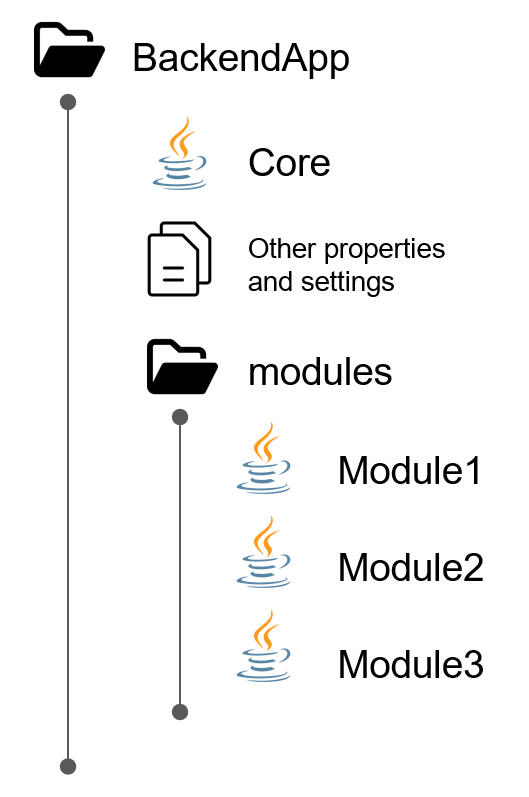
\includegraphics[scale=0.5]{images/plugin-folder-structure.png}
    \caption{Plugin architecture - Folder structure}
    \label{fig:figure1}
\end{figure}

\noindent In Figure \ref{fig:figure1}, the components labeled as core, module1, module2, and module3 represent packaged JARs. The core is responsible for detecting and loading the packaged Java sources from the modules folder. Typically, this task would require the use of a \textbf{ClassLoader}; however, Spring Boot simplifies this process for us. By utilizing Spring's loader properties \cite{springboot-loader-properties}, I can set the \hl{loader.path=file:modules/} property in the \textbf{loader.properties} file, located in the resources folder.
\\\\
The structure mentioned above presents various opportunities. For instance, in a distributed environment, if there's a need for a limited number of running instances but numerous lightweight microservices, instead of creating separate Spring Boot instances for each, they can all be appended to the same instance. Similarly, a small module responsible for logging or monitoring a specific microservice can be seamlessly integrated into the same instance. The environment can become even more dynamic if the loading and unloading of modules from the instance are controlled through commands given to the Spring Boot instance, such as REST API calls or periodic checks of a status flag inside each module, which can be externally updated.
\\\\
\noindent Ultimately, I concluded that continuing with this approach would introduce unnecessary complexity, especially since I didn't plan on adding numerous tightly coupled modules. Moreover, this strategy would necessitate the implementation of a plugin interface to specify the metadata of each service and an order loading mechanism to ensure that services dependent on others load after their dependencies are available.
\\\\
In the end, a simpler approach was chosen, but the above structure would still make an interesting choice in a more dynamic environment where there is a need for tightly coupled services that can be managed at runtime, using a plugin architecture.

\subsection{Final choice}


\noindent For this platform's use case, the final structure is organized as a \textbf{Maven project} with two Maven modules, thus adopting a \textbf{monolithic} approach. This approach simplifies the compilation and deployment of the modules within it. The parent pom defined in the main project allows for the specification of global parameters and configurations for shared dependencies. The modules themselves are implemented as \textbf{Spring Boot} projects, with one serving as a users microservice, functioning as an \textbf{authorization server}, and the other as a courses microservice (\textbf{resource server}), managing the official courses presented on the web platform. The authentication and authorization of resources is managed via \textbf{Spring Security}. Both Spring Boot applications are designed as \textbf{REST APIs}, following the \textbf{repository-service-controller pattern}.
\\\\
For the entire backend, I employ \textbf{Project Lombok} \cite{project-lombok}, a library that reduces code repetition and aids in writing cleaner code. An addition tool for boilerplate reduction is \textbf{MapStruct} \cite{mapstruct}, a library that generates mappers for classes automatically. For testing purposes, I utilize \textbf{JUnit} \cite{junit5} and \textbf{Mockito} \cite{baeldung-mockito}. Further details regarding library usage can be found in chapter \ref{Backend Explained}.

\newpage
\section{Frontend Framework}

Similar to the backend, my primary consideration for the frontend framework was focused on using a library with which I am familiar, specifically React.

\subsection{Initial attempts}

\noindent During my search for suitable frameworks, three names stood out to me: Vite (not a framework), Remix, and Next.js.

\subsubsection{Vite}

\noindent Vite, as described on its official website \cite{vite-guide}, is more of a frontend tool than a framework. It addresses common developer challenges by utilizing modern JavaScript features. With an integrated development server offering fast reloads and caching mechanisms, Vite significantly accelerates the development process. From what I have noticed, it is often chosen as an alternative to \textbf{Create React App}, boasting different bundling mechanics and notably faster performance. While Vite excels in client-side rendering, it lacks out-of-the-box support for server-side rendering, although this can be achieved through plugins.

\subsubsection{Remix}

\noindent After learning about Vite, I explored Remix, intrigued by its compatibility with Vite. According to their website \cite{remix-docs}, Remix is a framework built on top of React Router, serving as a compiler, server-side HTTP handler, server framework, and browser framework simultaneously. Although I see potential in Remix, particularly with its backing from Shopify, I faced challenges in finding necessary resources and specific use cases in their documentation. Consequently, I opted for a framework with a larger community, namely \textbf{Next.js}, as discussed in the final choice subsection.

\subsubsection{Modular frontend}

\noindent Regarding the frontend structure, I initially aimed for a modular approach, as I did for the backend. However, implementing this proved more challenging than anticipated. I considered utilizing monorepos as a solution, similar to the monolithic backend architecture. To manage this, I selected \textbf{Nx} \cite{nx-docs}, a build system designed for monorepos. Ultimately, navigating the complexities of Nx and its steep learning curve led me to abandon the idea of distinct microfrontends. Instead, I decided to only separate the modules structurally, as I considered it more suitable for my use case.

\subsection{Final choice}

\subsubsection{Why Next.js and not Remix}
\noindent Despite claims from one of Remix's co-founders that Remix matches, if not surpasses, Next.js in terms of speed \cite{remix-vs-next-according-to-remix}, I am inclined to favor Next.js for this web platform. While Remix may offer comparable performance, \textbf{Next.js} presents a larger ecosystem, providing abundant resources for specific use cases and ready-made solutions for common problems. Both Remix and Next.js are excellent solutions, but I personally found Next.js to be more accessible, both in terms of its features and documentation.
\\\\
\noindent Initially, I preferred Remix's routing approach, which allows you to specify all routes in the same file, whereas Next.js forces the usage of its file system route representation. This opinionated aspect initially concerned me, as I feared it would lead to a messy file hierarchy. However, in the end, I found this to be a beneficial standard, as it helps ensure that route segments remain manageable in length, by avoiding deep nesting. With the introduction of Next.js 13, a new App Router model was introduced, incorporating features such as Server Components, Streaming with Suspense, and Server Actions \cite{nextjs-app-router}. Although I initially used the Pages Router, I quickly migrated to the App Router to take advantage of its latest features. The transition was smooth, thanks to the documentation and support from the Discord community.

\subsubsection{Middleware}

\noindent One drawback of Next.js, in my view, is its tight integration of server and client aspects, which can occasionally lead to confusion about whether you are coding for the server side or client side of the application. Consequently, I have not considered using Next.js for the actual backend, preferring to keep the backend as a separate application. Therefore, the backend functionality of Next.js can be thought of as a \textbf{middleware} in the context of this web platform.

\subsubsection{Next.js Project}

\noindent The project was created using \hl{npx create-next-app@latest} \cite{nextjs-installation}, with \textbf{TypeScript}, \textbf{ESLint}, \textbf{Tailwind CSS} and \textbf{App Router} selected. On top of this, I also use \textbf{Prettier} \cite{prettier}, an opinionated code formatter in the Next.js project.
\\\\
\noindent \textbf{TypeScript} enhances code maintainability by introducing static typing to JavaScript variables. This allows the compiler and linter to detect potential issues such as incorrect type conversions or accessing undefined fields before they cause problems in production. Additionally, TypeScript enables text editors to provide context-aware suggestions based on variable types, leading to a more efficient development process. Since all TypeScript code is eventually compiled into JavaScript during the build process, there are no compatibility issues to worry about.
\\\\
\noindent \textbf{ESLint} is employed to enforce coding standards and maintain overall code quality. It identifies syntax errors, potential bugs, and problematic patterns, helping developers adhere to best practices and ensure consistency across the codebase.
\\\\
\noindent \textbf{Tailwind CSS} simplifies the project by eliminating the need for separate CSS files. Instead, styles are applied using predefined class names, reducing the overhead of managing custom class names and allowing for dynamic customization through class variants. Furthermore, Tailwind automatically removes unused styles during the bundling process, optimizing the CSS output.

\section{Frontend Optimization}

NextJS by itself already provides a lot of optimizations, such as automatic code splitting, image optimization, and server-side rendering. However, there are still some optimizations that can be done to improve the performance of the web platform.

\subsection{SWR}

\noindent SWR (stale-while-revalidate) is a strategy for caching data in the frontend, which is used for data that changes frequently. By using SWR, the web platform can display the latest data while also updating the cache in the background. This approach ensures that the user always has access to the most up-to-date information without sacrificing performance.
\\\\
\noindent Based on the previous invalidation strategy, a library with the same name, \textbf{SWR} \cite{swr}, is used. SWR is a React Hooks library for data fetching that provides out of the box ways to cache data, revalidate it, and handle errors. It is used on the client side to fetch data from the backend.

\section{Databases}

\subsection{H2 Database}

\noindent H2 \cite{h2} is a lightweight relational database management system, written in Java, which when used with Spring Boot, can be a fast solution for development and testing, as it acts as an in memory database. Since it supports SQL syntax, I am using it as a dummy database, executing the same queries I would for PostgreSQL, but without having to reset the database on each test instance.

\subsection{PostgreSQL}

\noindent PostgreSQL \cite{postgresql}, a relational database management system, is used for managing user data in this web platform. It handles critical information like personal details and refresh tokens. PostgreSQL was a top candidate when choosing, due to my prior experience with it, as well as its adherence to ACID principles, ensuring data integrity and reliability even under heavy user loads. Additionally, its open-source nature and permissive licensing model made it an attractive choice, especially compared to proprietary options like Oracle.
\\\\
\noindent The decision to use a relational database instead of a non-relational one was deliberate, considering the structured nature of the data and the need for a robust architecture to support complex relationships and transactions.

\subsection{MongoDB}

\noindent MongoDB \cite{mongodb} stands out as one of the preferred options for non-relational databases, especially in scenarios where data lacks a structured format. In the context of this web platform, a non-relational database was essential for managing course information due to its unstructured nature. Each course is represented as a JSON object with varying levels of depth, featuring a recursive structure of components that can nest within each other. MongoDB's capability to conduct full-text searches via specialized text indexes has proven to be a valuable asset. While it may not offer the complexity of search indexing seen in Elasticsearch, MongoDB's functionality proved sufficient for conducting course searches within the web application.

\subsection{Connecting to database}

\noindent Connection to the databases mentioned above is done through Spring Boot, especially through Spring Data \cite{spring-data}. For PostgreSQL and H2, I use Spring Data JPA with Hibernate, and also HikariCP \cite{hikaricp} for connection pooling. For MongoDB, Spring Data MongoDB is used.
\\\\
\noindent \textbf{JPA}, or Java Persistence API, serves as an interface defining standards for database manipulation, along with providing a native object-oriented query language known as JPQL.
\\\\
\noindent \textbf{Hibernate} is an implementation of the JPA guidelines, providing its own object-oriented query language as well, HQL.
\\\\
\noindent As Spring Data JPA is an integration for JPA, \textbf{Spring Data MongoDB} is an integration for MongoDB, offering a template helper class, data repositories, multiple document transactions and other useful features. 

\section{Deployment}

The web platform was designed with two profiles in mind: \textbf{development} and \textbf{production}. The development profile is intended for local testing and debugging, while the production profile is meant for deployment on a server. The deployment process is facilitated by \textbf{Docker} \cite{docker} and \textbf{Docker-Compose} \cite{docker-compose}, which allow for the creation of containers for the backend, frontend, and database. These containers are then orchestrated using Docker-Compose, ensuring that the web platform runs smoothly in a production environment.

\subsection{Running and Compiling}

\subsubsection{Backend}

\noindent For development purposes, the backend modules are run inside IntelliJ IDEA by executing the main class of each module. To run the modules successfully, some environment variables must be set. For this, a \textbf{.env} file is created in the root of each module, containing the necessary variables. A JetBrains plugin called \textbf{EnvFile} is used to load the environment variables from the .env file into the IDE. By default, the project is configured in Maven to use the \textbf{dev profile}.
\\\\
\noindent If the \textbf{prod profile} is selected, the modules can also be run using the above method, simulating a production environment. For example, it might be more accessible to test that the users module's production database (PostgreSQL) is running as expected, and there are no compatibility issues with the development database (H2), by running it directly in the IDE instead of compiling and testing outside it.
\\\\
\noindent After obtaining satisfying results with the previous method, the modules are compiled using Maven by running \hl{mvn clean package -P prod}, which generates a JAR file for each module using the \textbf{prod profile}. The JAR files are then run using the \hl{java -jar} command, with the necessary environment variables set.

\subsubsection{Frontend}

\noindent The frontend is run using the \hl{npm run dev} command, which starts the development server. The development server is accessible at \textbf{http://localhost:3000}. The frontend can also be run in production mode by running the \hl{npm run build} command, which compiles the NextJS project, followed by the \hl{npm run start} command. The production server is accessible at the same URL.
\\\\
\noindent The frontend also relies on environment variables, which are set in a \textbf{.env.local} file in the root of the frontend project and are automatically loaded by NextJS. Three files are used for environment variables: \textbf{.env.local} for local development, \textbf{.env.development} for development, and \textbf{.env.production} for production. Variables from the .env.local file have a higher priority, while the other two files are conditionally loaded based on the environment.
\\\\
\noindent \textbf{Attention!} NextJS will try to optimize many aspects of the application, but some of these optimizations might affect the behavior of the web platform. For example, NextJS caches all fetch requests by default, but this caching is not visible in development mode. If not careful, this might lead to unexpected results when testing the application, such as never-changing data, even if the backend has been updated.

\subsection{Docker}

\noindent Docker is a platform that simplifies the deployment process by packaging applications and their dependencies into containers. Containers are portable and isolated, ensuring that the contents run the same way in any environment. Docker also provides a centralized repository for storing and sharing container images, known as Docker Hub.
\\\\
\noindent To assist with the deployment process, a \textbf{Dockerfile} was created for each backend module, containing the necessary instructions for building the image. The Dockerfile for the backend modules is based on the \textbf{eclipse-temurin:17-jre-alpine} image and copies the compiled module JAR file into the image.
\\\\
\noindent The frontend also has a Dockerfile, based on the \textbf{node:18-alpine} image, with two stages: one for building the project and one for running it. The compiled project is copied into the second phase, which is then used to run the project. The frontend Dockerfile also contains the necessary instructions for installing the required dependencies and setting the environment variables.
\newpage
\noindent Although containers for the backend modules and frontend are created only for deployment, databases are needed in both development and production environments. For this reason, local containers were created and used for them. To visualize the data inside them, \textbf{pgAdmin} was used for PostgreSQL, and \textbf{mongo-express} for MongoDB.

\subsection{Docker-Compose}

\noindent Docker is a powerful tool for managing containers, but it can be challenging to orchestrate multiple containers manually, especially as the number of services increases.
\\\\
\noindent Docker-Compose is a tool for defining and running multi-container Docker applications. It simplifies the process of managing multiple containers by allowing users to define the services, networks, and volumes in a single file. The Docker-Compose file for the web platform contains the services for the backend, frontend, and database, as well as the necessary environment variables.
\\\\
\noindent The Docker-Compose file is used to build the images for the backend modules and frontend, as well as to create the containers for the database services. The containers are then started using the \hl{docker-compose up --build} command, which builds images and runs the services defined in the file. The web platform is accessible at \textbf{http://localhost:3000}.
\\\\
\noindent For communication between Docker services, a network is created by Docker-Compose, allowing the services to communicate with each other. Each service is accessible to the others by using the service name as the hostname, as defined in the Docker-Compose file.
\\\\
\noindent Tweaks can be made to the Docker-Compose file to modify the behavior of the services on a production server. For example, exposing specific ports, setting environment variables, or defining volumes for persistent data storage.

\subsection{Extending}

\noindent As the application grows, a CI/CD pipeline such as \textbf{Jenkins} can be implemented to automate the deployment process. This pipeline can be used to build, test, and deploy the application to a server, ensuring that the latest changes are always available to users. \textbf{Kubernetes} can also be used to manage the containers in a production environment, ensuring that the application is always available and scalable.